% Vorlage für eine Bachelorarbeit
% Siehe auch LaTeX-Kurs von Mathematik-Online
% www.mathematik-online.org/kurse
% Anpassungen für die Fakultät für Mathematik
% am KIT durch Klaus Spitzmüller und Roland Schnaubelt im Dezember 2011

\documentclass[11pt,a4paper,titlepage]{scrartcl}
% scrartcl ist eine abgeleitete Artikel-Klasse im Koma-Skript
% zur Kontrolle des Umbruchs Klassenoption draft verwenden

\usepackage{array}
% die folgenden Packete erlauben den Gebrauch von Umlauten und ß
% in der Latex Datei
\usepackage[utf8]{inputenc}
% \usepackage[latin1]{inputenc} %  Alternativ unter Windows
\usepackage[T1]{fontenc}
\usepackage[ngerman]{babel}
\usepackage[babel,german=quotes]{csquotes}
\usepackage[pdftex]{graphicx}
\usepackage{latexsym}
\usepackage{amsmath,amssymb,amsthm}
\usepackage[style=authoryear,backend=biber]{biblatex}
\usepackage{pdflscape}

%\bibliography{bib/test}


% Abstand obere Blattkante zur Kopfzeile ist 2.54cm - 15mm
\setlength{\topmargin}{-15mm}


% Umgebungen für Definitionen, Sätze, usw.
% Es werden Sätze, Definitionen etc innerhalb einer Section mit
% 1.1, 1.2 etc durchnummeriert, ebenso die Gleichungen mit (1.1), (1.2) ..

\newtheorem{Satz}{Satz}[section]
\newtheorem{Definition}[Satz]{Definition}     
\newtheorem{Lemma}[Satz]{Lemma}	
                  
\numberwithin{equation}{section} 

% einige Abkuerzungen
\newcommand{\C}{\mathbb{C}} % komplexe
\newcommand{\K}{\mathbb{K}} % komplexe
\newcommand{\R}{\mathbb{R}} % reelle
\newcommand{\Q}{\mathbb{Q}} % rationale
\newcommand{\Z}{\mathbb{Z}} % ganze
\newcommand{\N}{\mathbb{N}} % natuerliche

\title{Bachelorarbeit}
\author{Andre Weinkötz (14985714)}
\date{1. März 2018}


\begin{document}
  % Keine Seitenzahlen im Vorspann
  \pagestyle{empty}

  % Titelblatt der Arbeit
  \begin{titlepage}

\begin{center}
	\includegraphics[scale=0.20]{img/hm-logo.eps}
\end{center}
 \bigskip

 \begin{center} \large 
    
    Proposal zur Bachelorarbeit im Studiengang B.Sc. Wirtschaftsinformatik
    \vspace*{2.5cm}

    {\huge Proposal} \\ \vspace*{0.5cm}
   % Echtzeit-Anwendungen im Web durch WebSockets
    
    \vspace*{2.5cm}

    Andre Weinkötz \bigskip
    
    

    15. Oktober 2017
    \vspace*{2.5cm}
    
    

    Fakultät für Informatik und Mathematik \\
	Hochschule München\bigskip
	
	Betreuer: Prof. Dr. Mandl 
	
	
  \end{center}
\end{titlepage}


  % Inhaltsverzeichnis
 \tableofcontents

\newpage
%\textbf{ABSTRACT}
%\newpage
  % Ab sofort Seitenzahlen in der Kopfzeile anzeigen
  \pagestyle{headings}

\section{Motivation und Aufgabenstellung}
Die Anforderungen an Webanwendungen haben sich in den vergangenen Jahren stark verändert. Mobile Geräte wie Smartphones oder Tablets ersetzen stationäre Systeme, Webanwendungen sollen zur Kollaboration eingesetzt werden und Buchungssysteme oder Finanzanwendungen verlangen die Bearbeitung tausender Anfragen mit minimaler Verzögerung. Das Hypertext Transfer Protocol (HTTP) bietet hier keine zufriedenstellende Lösung. Um den Anforderungen an moderne Webanwendungen gerecht zu werden, spezifizierten das World Wide Web Consortium (W3C) und die Internet Engineering Taskforce (IETF) das WebSocket-Protokoll mit zugehöriger JavaScript-API. \\

\noindent Das Ziel der geplanten Bachelorarbeit ist der Einsatz dieser Technologie als didaktisches Mittel im Rahmen der Lehrveranstaltung “Web-Techniken” an der Hochschule München. Die Grundlage bildet dabei eine Chat-Anwendung aus der Lehrveranstaltung “Datenkommunikation”, die von den Studierenden im dritten Fachsemester als Studienarbeit bearbeitet wird.\\

 \noindent Zu Beginn werden die technischen Aspekte der WebSockets analysiert. Diese umfassen sowohl die konzeptionelle Spezifikation von WebSockets, als auch deren Implementierung in Java. Dabei sollen traditionelle Webtechniken und das neue Konzept gegenübergestellt werden, um die jeweiligen Vor- und Nachteile aufzuzeigen. Zusätzlich wird untersucht, welche Anwendungsfälle das größte Potential bei dem Einsatz von WebSockets bergen. \\
 
 \noindent Der Kern der Arbeit handelt vom Umbau der bestehenden Anwendung. Hier soll eine Analyse der bestehenden Anwendung erfolgen, um daraus die Anforderungen an die modifizierte Version abzuleiten. Die Umsetzung dieser Anforderungen erfolgt zunächst konzeptionell und wird anschließend  unter Berücksichtigung des erstellten Konzepts implementiert. Als serverseitige Programmiersprache wird Java beibehalten. Der Programmteil zur Leistungsmessung wird ebenfalls in Java verfasst. Die Implementierung der clientseitigen Chat-Anwendung erfolgt in JavaScript.\\
 
\noindent Zum Einsatz der Anwendung im Rahmen einer Lehrveranstaltung wird ein Lehrkonzept erstellt, das als zukünftige Aufgabenstellung oder Anleitung fungiert. Abschließend wird die Leistungsfähigkeit beider Anwendungen geprüft und bewertet. Zudem wird der Einsatz der modifizierten Anwendung als interaktive Methode einer Lehrveranstaltung evaluiert.

\section{Methodik und Durchführung}
Um die genannten Ziele zu erreichen, kommen verschiedene Methoden zum Einsatz. Die Analyse der technologischen Aspekte folgt dabei argumentativ-deduktiven Grundsätzen. Der Hauptteil der Arbeit orientiert sich an den Methoden des Software Engineerings nach Balzert. 
 
 \paragraph{Anforderungsanalyse und -definition}Die Anforderungen an die zu entwickelnde Anwendung werden zunächst systematisch ermittelt und spezifiziert sowie anschließend nach Rücksprache validiert und abgenommen. 
 \paragraph{Entwurf und Prototyping}Die Ergebnisse der Analyse werden konzeptionell durch den Einsatz standardisierter Darstellungsformen aufbereitet und prototypisch implementiert. Der explorative Prototyp dient zur Validierung sowohl der Grundidee als auch der Akzeptanz innerhalb der Zielgruppe. Diese wird durch ausgewählte Studierende des dritten Semesters repräsentiert. Anhand einer vorläufigen Aufgabenstellung testen sie den Prototyp und melden ihre Eindrücke über einen Fragebogen zurück. So soll der qualitative Mehrwert der Anwendung als Lehrmittel sichergestellt werden.
 \paragraph{Implementierung und Evaluierung}
Unter Berücksichtigung dieser Erkenntnisse wird die Architektur der bestehenden Anwendung hinsichtlich der Verwendung von WebSockets überarbeitet. Abschließend erfolgt die Evaluierung der Leistungsfähigkeit beider Anwendungen in einer kontrollierten Testumgebung.


\section{Erwartete Ergebnisse und Ausblick}
Das Ergebnis dieser Bachelorarbeit besteht aus zwei Teilen.\\

 Der erste Teil umfasst die modifizierte Chat-Anwendung auf Basis von WebSockets sowie eine ausführliche Dokumentation. Der Autor erwartet durch den Leistungsvergleich festzustellen, dass die Antwortzeiten beider Anwendungen nur geringfügig voneinander abweichen. Dadurch soll belegt werden, dass Anwendungen, welche bisher ein TCP-basiertes Client-Server-Modell benötigten, durch die WebSocket Technologie ersetzt werden können.\\

Der zweite Teil besteht aus den Ergebnissen der Fragebögen des Prototyp-Tests sowie der Ausarbeitung einer Aufgabenstellung für Studierende. Die Aufgabenstellung soll den Themenbereich der WebSockets strukturieren und so aufbereiten, dass Studierende diesen nach ausreichender Übung verstehen und selbst anwenden können. Der Autor erhofft sich dadurch, den Einstieg in neue Bereiche der Webentwicklung für Studierende zu erleichtern.\\ 		

\noindent Diese Bachelorarbeit und insbesondere die modifizierte Chat-Anwendung können auch als Basis für weitere Projekte genutzt werden. So ist es denkbar, dass im Rahmen einer größeren Studienarbeit eine komplexe Webanwendung entwickelt werden soll, in welche die Chat-Anwendung integriert wird. Ebenfalls besteht die Möglichkeit die Chat-Anwendung zu erweitern, indem neue Frameworks wie Angular zur Darstellung von Webanwendungen eingesetzt werden.

\section{Sonstige Inhalte}
\subsection{Vorläufige Gliederung}
In Abbildung \ref{fig:toc} ist die vorläufige Struktur dargestellt. Die Einleitung führt in die Thematik der WebSockets ein und beschreibt deren Notwendigkeit. Das zweite Kapitel enthält weiterführende Informationen zur WebSocket-Technologie. Im dritten und vierten Kapitel wird der Umbau der ChatApplikation mittels Methoden des Software Engineerings beschrieben. Im fünften Kapitel findet die Evaluation statt. Das letzte Kapitel fasst die Bachelorarbeit zusammen und gibt einen Ausblick auf mögliche weitere Projekte oder Anwendungsmöglichkeiten.
\begin{figure}[ht] \label{fig:toc}
	\begin{center}
	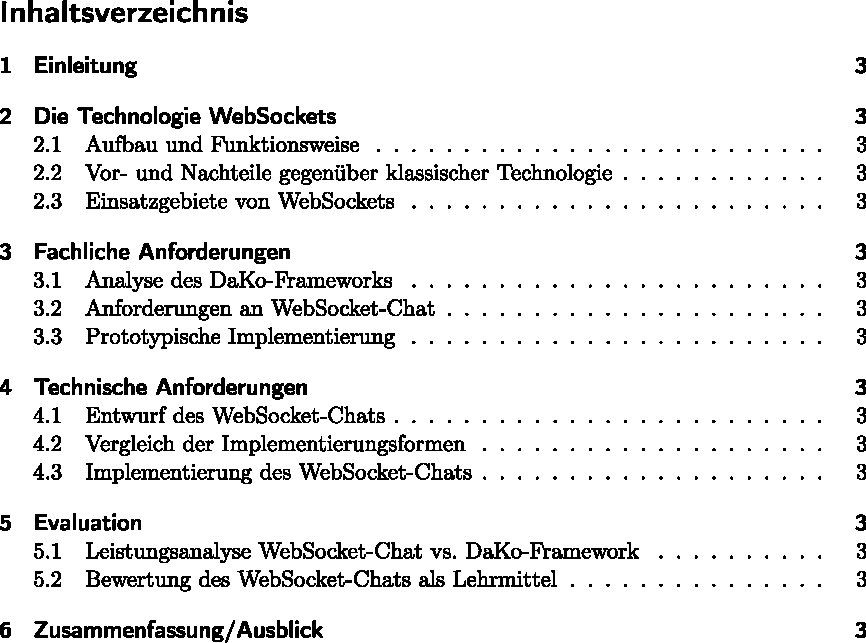
\includegraphics[scale=1.0]{img/toc.pdf}
		 \caption{Vorläufiges Inhaltsverzeichnis}
	\end{center}
\end{figure}

Dieses Inhaltsverzeichnis wird im Laufe der Bachelorarbeit verändert, erweitert und detaillierter gestaltet.

\newpage
	\subsection{Projektplan}
	Der beiliegende Projektplan startet am 30. Oktober 2017 mit der Vorbereitungsphase. In dieser Phase wird die erforderliche Literatur ermittelt und ausgewertet. Dies erfolgt immer in Rücksprache mit Herrn Prof. Dr. Mandl.  Abgeschlossen wird diese Phase mit der offiziellen Anmeldung der Bachelorarbeit am 28. November 2017. In der Strukturierungsphase wird eine detailliertere Gliederung erstellt und die Informationen aus der Literatur strukturiert. In der Schreibphase wird neben der schriftlichen Fassung auch die Programmierung des Quellcodes durchgeführt. Einzelne Kapitel oder Teile des Programms werden Herrn Prof. Dr. Mandl zur Kontrolle bereitgestellt. Abschließend werden Korrekturen eingearbeitet und die Bachelorarbeit am 28. Februar 2017 offiziell eingereicht.
	\begin{figure}[ht] \label{fig:tt}
		\begin{center}
			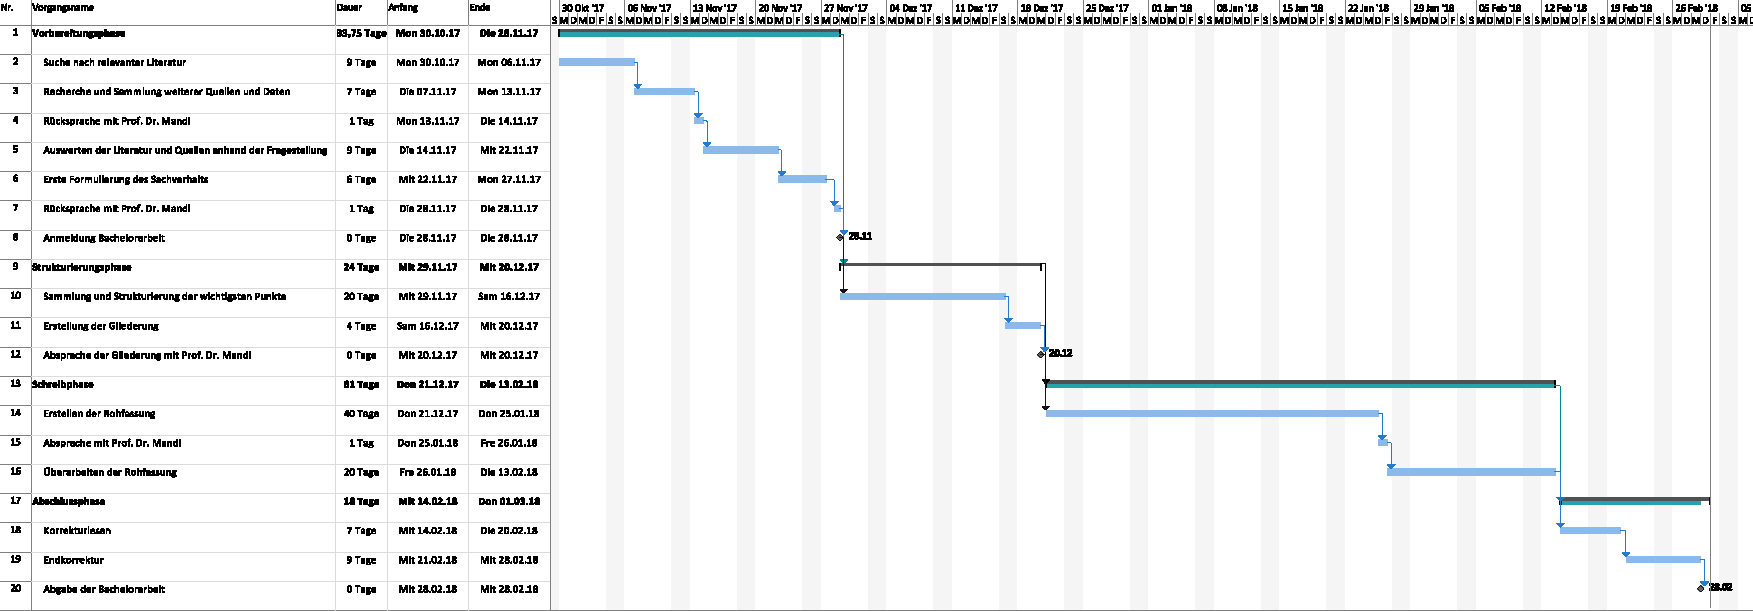
\includegraphics[scale=0.5]{img/tt.pdf}
			\caption{Zeitplan}
		\end{center}
	\end{figure}

Der Zeitplan soll lediglich als grobe Orientierung dienen. Regelmäßige Absprachen mit Herrn Prof. Dr. Mandl sind geplant, jedoch sind hierfür noch keine Termine festgelegt.  
\newpage
\subsection{Vorläufiges Literaturverzeichnis}
	\begin{figure}[!ht] \label{fig:vz}
	\begin{center}
		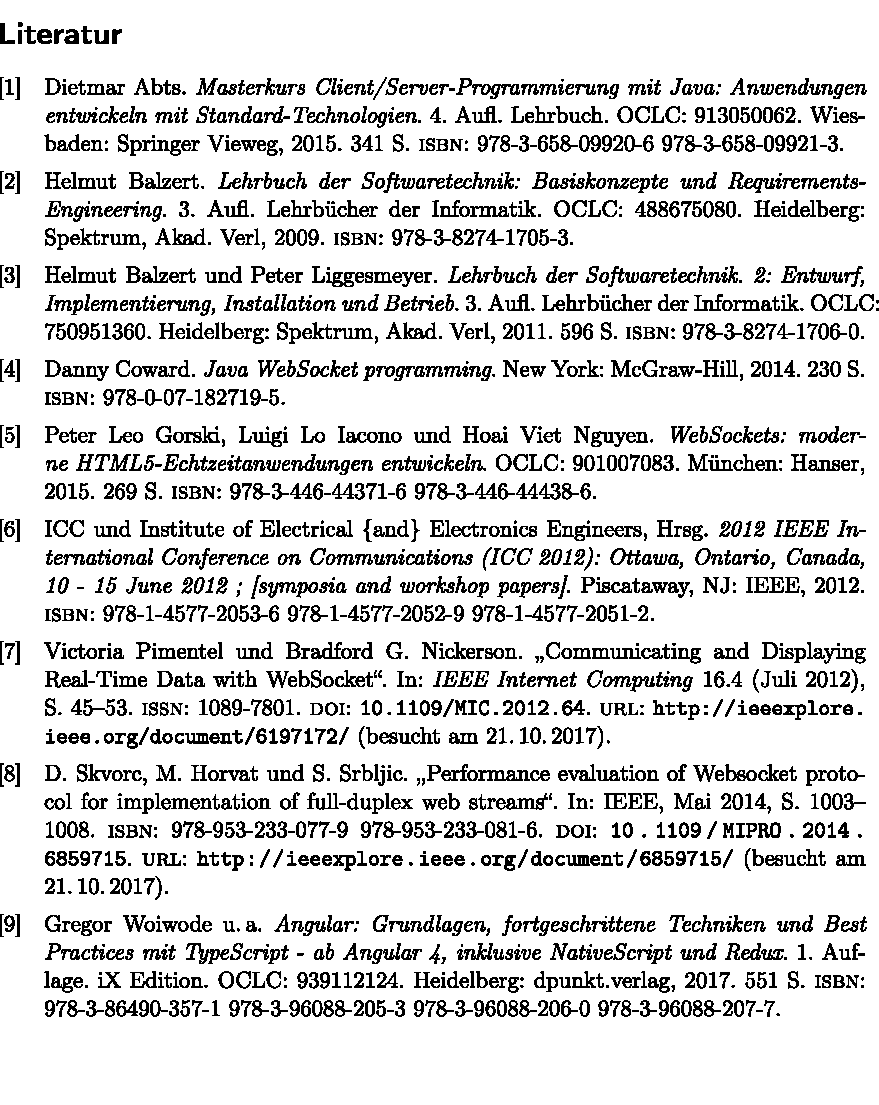
\includegraphics[scale=0.9]{img/vorlvz.pdf}
		\caption{Vorläufiges Literaturverzeichnis}
	\end{center}
\end{figure}

% Unterschrift (handgeschrieben)

%\newpage

%\printbibliography

%\newpage
%\listoffigures
%\listoftables

\end{document}
